%% GENERATED by tools/from_docs.py from stepss-docs. Do not edit by hand:
%% edit the page named below in stepss-docs and regenerate.
%% source: stepss-docs/src/content/docs/python/examples.md

\chapter{Python examples}\label{doc:py-examples}

All examples assume the working directory contains the relevant data and disturbance files.

\section{Running a Basic Simulation}\label{py-examples:running-a-basic-simulation}

Define the test case, run the simulation, and extract results:

\begin{Verbatim}
import stepss

case = stepss.cfg()
case.addData('dyn_A.dat')        # dynamic models
case.addData('volt_rat_A.dat')   # power-flow initialisation
case.addData('settings1.dat')    # solver settings
case.addDst('short_trip_branch.dst')
case.addInit('init.trace')
case.addTrj('output.trj')        # save trajectories for post-processing
case.addObs('obs.dat')           # define which observables to record
case.addCont('cont.trace')
case.addDisc('disc.trace')
case.addRunObs('BV 4044')        # record bus voltage while the run proceeds
case.addRunObs('BV 1041')
case.writeCmdFile('cmd.txt')     # save for future reuse

ram = stepss.sim()
ram.execSim(case)                # run to completion

ext = stepss.extractor(case.getTrj())
ext.getBus('1041').mag.plot()    # voltage magnitude at bus 1041
\end{Verbatim}

\begin{docsnote}{Note}

Set \texttt{\$NB\_THREADS\ 0\ ;} in the solver settings file to use all available CPU cores
for parallel simulation. The free version uses at most \textbf{2 cores} whatever this
is set to; a \texttt{\$LICENSE} record in the data files lifts the cap. See
\hyperref[ch-legal]{License}.

\end{docsnote}

\section{Pause and Continue}\label{py-examples:pause-and-continue}

Pause the simulation at intermediate time points to inspect state or add disturbances:

\begin{Verbatim}
ram = stepss.sim()
ram.execSim(case, 0.0)                        # initialise, paused at t=0
ram.contSim(10.0)                             # simulate to t=10 s
ram.contSim(ram.getSimTime() + 60.0)          # advance 60 s from current time
ram.contSim(ram.getInfTime())                 # run to end of time horizon
\end{Verbatim}

\section{Querying System State}\label{py-examples:querying-system-state}

Query bus voltages, branch flows, observables, and parameters while paused:

\begin{Verbatim}
ram.execSim(case, 10.0)

# Bus voltages
busNames = ['g1', 'g2', 'g3']
voltages = ram.getBusVolt(busNames)   # list of voltage magnitudes (pu)
phases   = ram.getBusPha(busNames)    # list of phase angles (deg)

# Branch power flows
branch_pq = ram.getBranchPow(['1041-01'])  # [[P_from, Q_from, P_to, Q_to]]

# Component observables: P of injector L_11, vf of exciter g2, Pm of governor g3
comp_type = ['INJ',  'EXC', 'TOR']
comp_name = ['L_11', 'g2',  'g3']
obs_name  = ['P',    'vf',  'Pm']
obs = ram.getObs(comp_type, comp_name, obs_name)

# Component parameters: V0 of exciter g1, KPSS of exciter g2
comp_type = ['EXC', 'EXC']
comp_name = ['g1',  'g2']
prm_name  = ['V0',  'KPSS']
prms = ram.getPrm(comp_type, comp_name, prm_name)

# All component names of a type
all_buses = ram.getAllCompNames('BUS')
all_gens  = ram.getAllCompNames('SYNC')
\end{Verbatim}

\section{Adding Disturbances at Runtime}\label{py-examples:adding-disturbances-at-runtime}

Inject disturbances and parameter changes while the simulation is running:

\begin{Verbatim}
ram.execSim(case, 80.0)

# LTC voltage setpoint changes at t=100 s (ramp)
for i in range(1, 6):
    ram.addDisturb(100.0, f'CHGPRM DCTL {i}-104{i}  Vsetpt -0.05 0')

# Fault and clearance
ram.addDisturb(100.0, 'FAULT BUS 4032 0. 0.')         # 3-phase short circuit
ram.addDisturb(100.1, 'CLEAR BUS 4032')                # clear fault
ram.addDisturb(100.1, 'BREAKER BRANCH 4032-4044 0 0')  # trip line

# Generator trip
ram.addDisturb(100.0, 'BREAKER SYNC_MACH g7 0')

ram.contSim(ram.getInfTime())
\end{Verbatim}

For full disturbance syntax, see the \hyperref[ch-disturb]{Disturbances reference}.

\section{Plotting Results}\label{py-examples:plotting-results}

Extract and plot time-series results after the simulation:

\begin{Verbatim}
import stepss
ext = stepss.extractor('output.trj')

# Single curve
ext.getSync('g5').S.plot()       # rotor speed of generator g5
ext.getBus('4044').mag.plot()    # voltage magnitude at bus 4044

# Multiple curves on the same plot
curves = [ext.getSync(f'g{i}').S for i in range(1, 5)]
stepss.curplot(curves)

# Exciter and governor outputs
ext.getExc('g1').vf.plot()       # field voltage
ext.getTor('g1').Pm.plot()       # mechanical power

# Branch power flows
ext.getBranch('1041-01').PF.plot()

# Injector (wind/PV/BESS)
ext.getInj('WT1a').Pw.plot()

# Two-port (HVDC)
ext.getTwop('hvdc1').P1.plot()
\end{Verbatim}

Every one of those calls opens a matplotlib figure. Run against the bundled
Kundur two-area example, whose disturbance steps load \texttt{L9} at \texttt{t\ =\ 1\ s}, the
first three look like this.

\texttt{ext.getSync(\textquotesingle{}G1\textquotesingle{}).P.plot()}, one curve, labelled from the trajectory:

\begin{figure}[htbp]
\centering
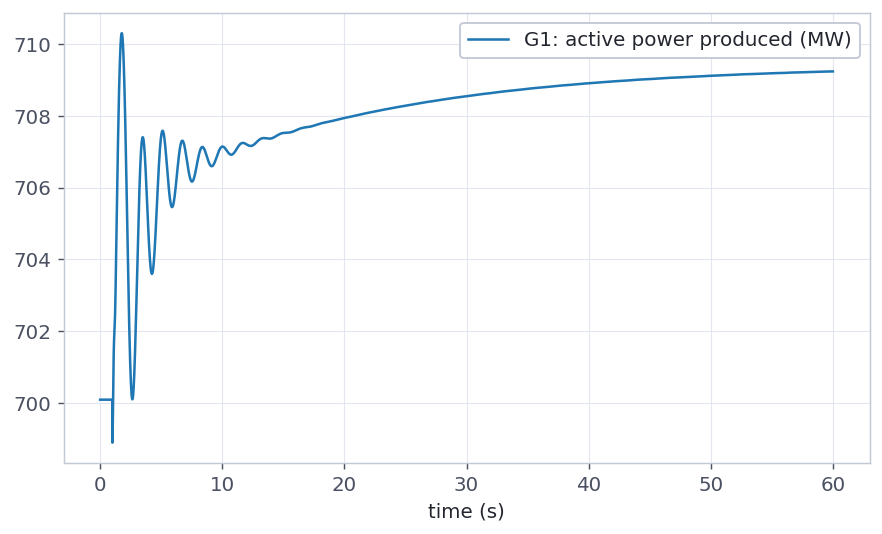
\includegraphics[width=0.85\linewidth]{figures/py-plot-single-light}
\caption{Active power produced by generator G1 against time, in megawatts over 60 seconds.}
\end{figure}

\texttt{stepss.curplot({[}...{]})}, several curves on one set of axes. Putting all four
machines together is what separates the areas: \texttt{G3} starts 19 MW above the rest
and stays there, while \texttt{G1}, \texttt{G2} and \texttt{G4} sit on top of one another.

\begin{figure}[htbp]
\centering
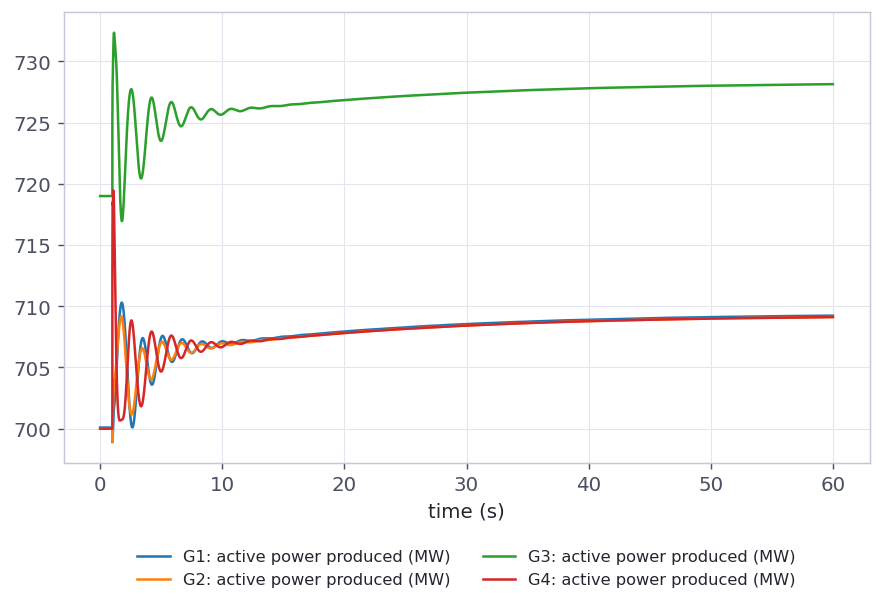
\includegraphics[width=0.85\linewidth]{figures/py-plot-multi-light}
\caption{Active power produced by generators G1 to G4 against time, four curves on one set of axes with a legend below them.}
\end{figure}

\texttt{ext.getBus(\textquotesingle{}9\textquotesingle{}).mag.plot()}, the same run seen as a voltage rather than a
power:

\begin{figure}[htbp]
\centering
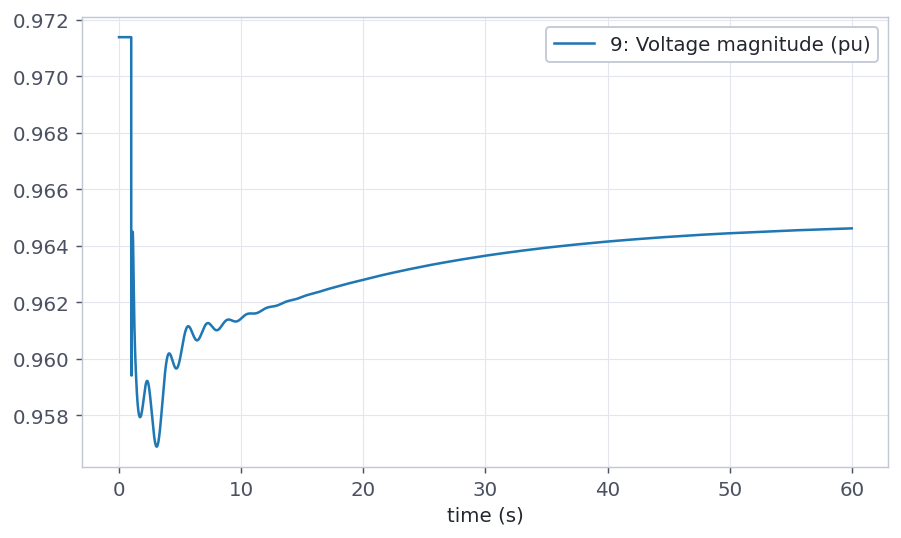
\includegraphics[width=0.85\linewidth]{figures/py-plot-bus-light}
\caption{Voltage magnitude at bus 9 against time, in per unit over 60 seconds.}
\end{figure}

These are ordinary matplotlib figures, so the usual \texttt{savefig}, styling and
subplot handling all apply to them.

\section{Live Plotting}\label{py-examples:live-plotting}

Watch chosen quantities as the simulation computes them, one panel per
observable:

\begin{Verbatim}
import stepss

ram = stepss.sim()
ram.execSim(case, 0.0)                   # initialise, paused at t = 0

mon = stepss.monitor(ram, [
    'BV 4044',                           # voltage magnitude of bus 4044
    'MS g6',                             # rotor speed of machine g6
    'BPO 4041-4044',                     # active power at the branch origin
    'RT RT',                             # wall clock, to gauge simulation speed
], title='Nordic')

curves = mon.run(step=0.1)               # to the end of the scenario
mon.savefig('live.png')
\end{Verbatim}

Each observable gets a panel, the panels share the time axis, and the figure is
redrawn as the run advances. \texttt{RT\ RT} is the one to include when you want to see
how fast the run itself is going: a straight line means the engine is keeping a
steady pace, and a knee in it is where the case got expensive.

\begin{figure}[htbp]
\centering
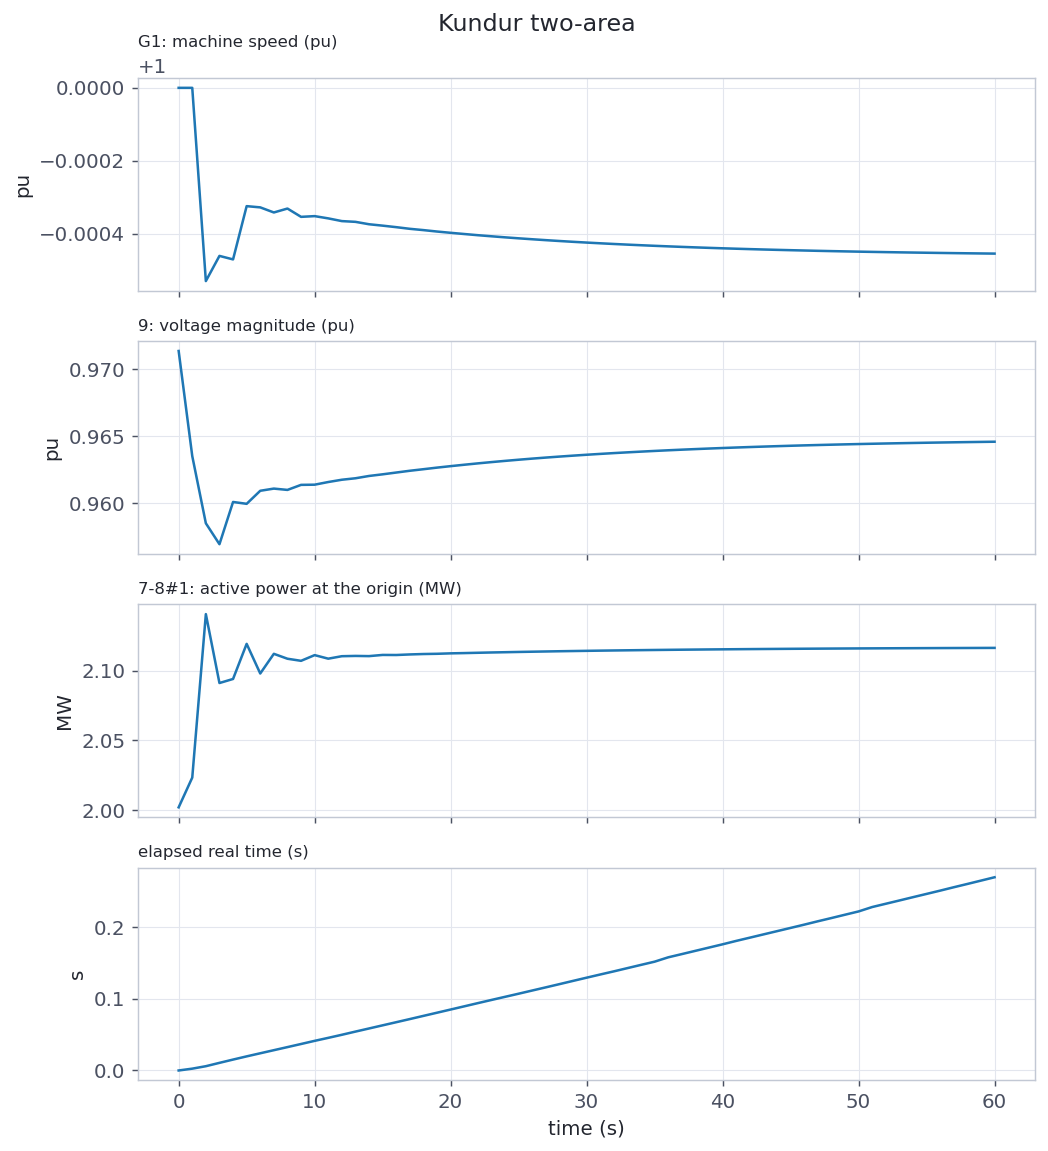
\includegraphics[width=0.85\linewidth]{figures/py-monitor-light}
\caption{A live monitor figure titled Kundur two-area, four panels stacked on a shared time axis running to 60 seconds.}
\end{figure}

\texttt{run} returns the same \texttt{cur} objects the extractor produces, so the collected
data goes straight into the post-processing above:

\begin{Verbatim}
stepss.curplot(curves)
\end{Verbatim}

Drive the stepping yourself when the run needs disturbances injected along the
way:

\begin{Verbatim}
mon = stepss.monitor(ram, ['BV 4044', 'BV 1041'])
for target in range(10, 200, 10):
    ram.contSim(float(target))
    mon.sample()
    mon.refresh()
    if target == 100:
        ram.addDisturb(105.0, 'CHGPRM DCTL 1-1041 Vsetpt -0.05 0')
\end{Verbatim}

\section{Parameter Sweep}\label{py-examples:parameter-sweep}

Run multiple simulations with varying parameters and collect results:

\begin{Verbatim}
import stepss
import numpy as np

results = {}
for disturbance_time in [5.0, 10.0, 20.0]:
    case = stepss.cfg('cmd.txt')
    trj_file = f'output_{disturbance_time:.0f}.trj'
    case.addTrj(trj_file)
    case.addObs('obs.dat')

    ram = stepss.sim()
    ram.execSim(case, 0.0)
    ram.addDisturb(disturbance_time, 'BREAKER SYNC_MACH g7 0')
    ram.contSim(ram.getInfTime())
    ram.endSim()

    ext = stepss.extractor(trj_file)
    min_freq = np.min(ext.getSync('g5').S.value)
    results[disturbance_time] = min_freq
    print(f't_dist={disturbance_time:5.1f}s  min_speed={min_freq:.5f} pu')
\end{Verbatim}

\section{Eigenanalysis Workflow}\label{py-examples:eigenanalysis-workflow}

RAMSES performs the small-signal analysis itself. Schedule an \texttt{EIG} event at the
operating point and it writes the modes, participation factors and mode shapes:

\begin{Verbatim}
import stepss

case = stepss.cfg('cmd.txt')
ram = stepss.sim()

ram.execSim(case, 0.0)               # pause at the steady-state operating point
ram.addDisturb(0.001, "EIG 'ssa'")   # writes ssa_modes.dat, ssa_pf.dat, ssa_ms.dat
ram.contSim(0.01)                    # advance past the event so it fires
ram.endSim()
\end{Verbatim}

Reading the result needs nothing beyond numpy:

\begin{Verbatim}
import numpy as np

m = np.loadtxt('ssa_modes.dat', comments='#')
freq, zeta = m[:, 4], m[:, 3]

interarea = m[(freq > 0.4) & (freq < 0.9) & (m[:, 2] > 0)]
print('inter-area mode: %.4f Hz, zeta = %+.4f' % (interarea[0, 4], interarea[0, 3]))
\end{Verbatim}

A complete annotated walkthrough ships with the package under
\texttt{examples/eigenanalysis/}.

\textbf{To drive your own solver instead}, \texttt{getJac()} returns the descriptor-form pair
as SciPy sparse matrices. This is the route for systems above \texttt{\$EIG\_MAX\_STATES},
where the engine's dense solve is not practical and sparse shift-invert methods
are needed:

\begin{Verbatim}
ram.execSim(case, 0.0)
A, E = ram.getJac()   # scipy.sparse.csc_matrix
ram.endSim()
\end{Verbatim}

\begin{docsnote}{Note}

Both routes need \texttt{\$OMEGA\_REF\ SYN\ ;} and \texttt{\$SCHEME\ DE\ ;} in the solver settings.
\texttt{EIG} refuses without them, exiting 78 with the reason in the log; the \texttt{JAC}
export skips with a warning under COI. See
\hyperref[doc:eigenanalysis]{Eigenanalysis}.

\end{docsnote}

\section{Test System Examples}\label{py-examples:test-system-examples}

The following examples use the ready-to-run test systems. For system descriptions, data files, and disturbance scenarios, see the \hyperref[doc:ts-index]{Test Systems} section.

\subsection{Nordic Test System: Generator Trip}\label{py-examples:nordic-test-system-generator-trip}

Trips generator g7 at \(t = 10\) s on the heavily-stressed Operating Point B and observes the voltage collapse dynamics over 150 seconds. See the \hyperref[doc:ts-nordic]{Nordic Test System} page for full system details and file descriptions.

\begin{Verbatim}
import stepss
import os

case = stepss.cfg()
case.addData('dyn_B.dat')
case.addData('volt_rat_B.dat')
case.addData('settings1.dat')
case.addDst('nothing.dst')
case.addObs('obs.dat')
case.addTrj('output.trj')

for f in os.listdir('.'):
    if f.endswith('.trj') or f.endswith('.trace'):
        os.remove(f)

ram = stepss.sim()
ram.execSim(case, 0.0)
ram.addDisturb(10.0, 'BREAKER SYNC_MACH g7 0')
ram.contSim(150.0)
ram.endSim()

ext = stepss.extractor(case.getTrj())
ext.getSync('g7').S.plot()    # rotor speed
ext.getBus('1041').mag.plot()  # voltage at central bus
\end{Verbatim}

\subsection{5-Bus System: Exciter Parameter Change}\label{py-examples:bus-system-exciter-parameter-change}

Applies a step change to the exciter voltage setpoint at \(t = 1\) s and plots the generator response. See the \hyperref[doc:ts-5bus]{5-Bus Test System} page for details.

\begin{Verbatim}
import stepss
import os

case = stepss.cfg()
case.addData('dyn.dat')
case.addData('lf1solv.dat')
case.addData('solveroptions.dat')
case.addDst('nothing.dst')
case.addObs('obs.dat')
case.addTrj('output.trj')

for f in os.listdir('.'):
    if f.endswith('.trj') or f.endswith('.trace'):
        os.remove(f)

ram = stepss.sim()
ram.execSim(case, 0.0)
ram.addDisturb(1.0, 'CHGPRM EXC G Vo 0.05 2')
ram.contSim(60.0)
ram.endSim()

ext = stepss.extractor(case.getTrj())
ext.getSync('G').P.plot()
ext.getSync('G').Q.plot()
\end{Verbatim}

The exciter set point rises by 0.05 pu, so the machine's reactive output is what
moves: active power holds at its scheduled 450 MW while reactive power climbs
from 68 to about 120 Mvar in a couple of seconds and settles there.

\begin{figure}[htbp]
\centering
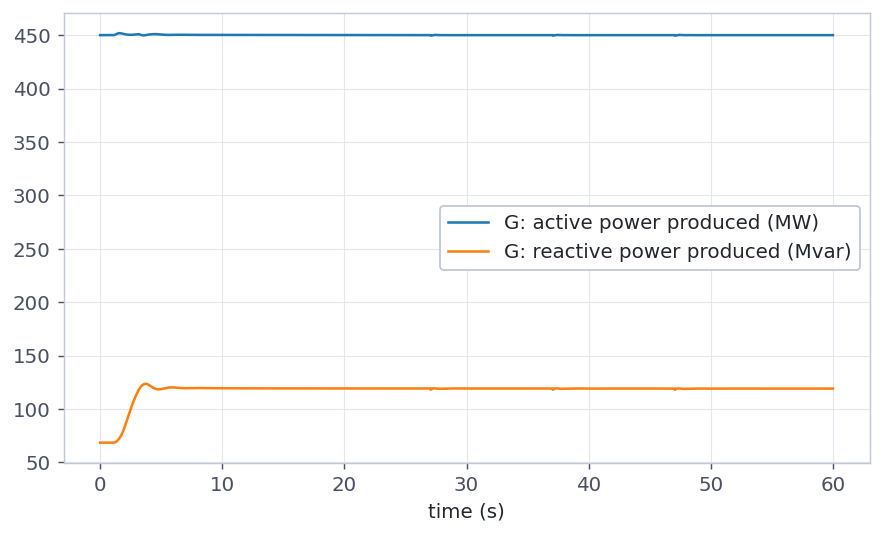
\includegraphics[width=0.85\linewidth]{figures/py-five-bus-exciter-light}
\caption{Active and reactive power produced by the 5-bus system's single generator against time, over 60 seconds.}
\end{figure}
